

\subsection{Real Data Example }%\color{red}we only report results by our method\color{black}
\label{realData}
\subsubsection{Data description }We use daily settlement European call option prices written on the underlying DAX 30 stock index. The sample spans the period between January 2, 2002 and December 3, 2011 and includes a total of 2557 days. The option prices are computed at the end of the trading day by EUREX based on the recorded intraday transaction prices. %The data set was accessed through the Research Data Center (RDC) at the CRC 649. 
The expiration dates for the options are set on every third Friday of a month. Therefore, only option prices with a few maturities are available on a particular day, see Figure~\ref{exp}. The distance between two consecutive maturities is increasing with the maturity, while the distance between two consecutive strikes for the settlement option prices is relatively constant. This data structure, with only a few available maturities daily, still allow the use of local polynomial method for smoothing in our application because the estimates in the maturity direction can be interpreted as weighted averages of the neighboring estimates for fixed observed maturities. This is similar to interpolation that is often used in practice for option prices. %For this data structure containing sparse areas for high maturities, the nearest-neighbor interpolation method introduces potentially high bias since the call options are known to vary monotonically with the strike and the expiration date. Therefore, we choose instead the linear interpolation to get the curves on the common grid. In this setup, this gives better results in finite sample than the nearest neighborhood method. 
We include call options with maturity between one day and one year. Our sample contains prices of options with an average of six maturities and sixty-five strikes per day. % From these data we We don't use all these data because of truncations requited by finding the maximum overlapping domain over all curves.

We assume 'sticky' coordinates for the daily observations, see equation \eqref{q10}, and standardize both the strike and the call prices within one day by the forward stock index value to ensure that the observations are in the same range. %the observed options occur on the same range of relative strikes, that is our moneyness metrics $m$. %\color{red}Observations of each curve $C_i$ no longer occur at the same grid points. We use nearest neighborhood (in moneyness direction) and linear (in maturity direction) interpolation to compute the values of the call prices on an equidistant grid defined as the maximum common domain of observations in both dimensions. Our choice for the interpolation points is: thirty-one distinct grid points for the moneyness and twenty for the maturity. For simplicity, we treat them as direct observations further on. Consequently, we apply the FPCA to noisy standardized call prices and estimate their second derivative with respect to $m$ in a fixed design setup.\color{black}
%(The treatment of random design was already discussed in section.)%$T=[  \underset{t}{\left\{ \operatorname{max}} \left(\underset{j}{\operatorname{min}} R_{t,j}\right) \right\} ]x[]$.  
%In order to retrieve the estimated SPDs we also need risk free interest rate daily data for various maturities, see equation \eqref{q09}. We derive a proxy for these based on the term structure of the LIBOR rate. We compute the corresponding annual interest rate by linearly interpolating the available LIBOR rates on a daily base. 
%In the real data application we do not pre-multiply the daily observations with the corresponding $\exp{(r_{i,\tau},\tau)}$  in equation (\ref{q09}) and report the results of the FPCA decomposition in terms of equation (\ref{q}). %The implicit assumption is that for the considered time frame the risk free interest rate is constant. 
Following the methodological framework, we apply the FPCA to the rescaled call prices and report the decomposition results for their second derivative with respect to moneyness. %As a consequence, the estimated components have not been adjusted to account for the interest rate term structure in the maturity direction and its daily variability is incorporated in the loadings. To obtain the SPD on a particular day $i$ we need to multiply the second derivative of the call prices obtained from a reduced form model by $\exp{(r_{i,\tau}\tau)}$ for each maturity $\tau$, see equation (\ref{q09}). If one is interested in the SPD dynamics rather than in the call derivative, an alternative to this procedure is to pre-multiply the daily call observations by the corresponding discount factors
%$\exp{(r_{i,\tau},\tau)}$ 
%and afterwards apply FPCA to the adjusted prices. Each choice is best fitted to a particular research goal.
%For illustrating our framework and for the purpose of comparing our results with the empirical literature on the implied volatility surfaces we considered the first approach better suited. 
Our proxy for the risk-free
interest rates are the EURIBOR rates, which are listed daily for several maturities. We perform a linear interpolation to calculate the rate values for the desired maturities.% variation of the interest rate can be corrected for subsequently, if one is interested in the shape of the SPD on a particular. 
%This is achieved by considering daily yield term for discounting in the moneyness direction. 

%We do not pre-multiply the daily observations with the corresponding $\exp{(r_{i,\tau},\tau)}$  in equation (\ref{q09})


         
\begin{table}[ht]
\begin{center}
\begin{tabular}{c|r@{.}l  r@{.}l  r@{.}l  r@{.}l  r@{.}l  r@{.}l  r@{.}l  r@{.}l  r@{.}l  r@{.}l}\hline\hline      $r$,     $L_{\max}$ &\multicolumn{2}{c}{1}&\multicolumn{2}{c}{2}&\multicolumn{2}{c}{3}&\multicolumn{2}{c}{4}&\multicolumn{2}{c}{5}&\multicolumn{2}{c}{6}&\multicolumn{2}{c}{7}&\multicolumn{2}{c}{8}&\multicolumn{2}{c}{9}&\multicolumn{2}{c}{10}\\ \hline
  %\multicolumn{2}{c}{r=1}&\multicolumn{2}{c}{r=2}&\multicolumn{2}{c}{r=3}&\multicolumn{2}{c}{r=4}&\multicolumn{2}{c}{r=5}&\multicolumn{2}{c}{r=6}&\multicolumn{2}{c}{r=7}&\multicolumn{2}{c}{t=8}&\multicolumn{2}{c}{r=9}&\multicolumn{2}{c}{r10}\\ \hline
 $\lambda_r\times 10^{6}$&  133&29 & 18&90 &  2&69&  1&62 &  0&49 &  0&34 &  0&26  & 0&09 &  0&08  & 0&05\\
  % $\lambda_r\times 10^{6}$&  144&49 & 12&00 &  4&36 &  1&08  &  0&87 &  0&37 &  0&17  & 0&14 &  0&08  & 0&03\\
 % $\lambda_r^{(d)}\times 10^{6}$&   63&66 & 23&86 &  6&77 & 4&81 &  2&47 &   1&03  &  0&78  &  0&57  &  0&54  & 0&41\\  \hline
  $\lambda_r^{(d)}\times 10^{2}$&   14&74 & 3&76 &  2&83 & 2&14 &  1&12 &   0&80  &  0&20  &  0&19  &  0&515  & 0&12\\  \hline  
 % $\lambda_r /  \lambda_{r+1}$&   12&04  &  2&76  &  4&02  &  1&25 &  2&37 &  2&15 & 1&20  & 1&81  &  2&47 &  1&26\\
   $\lambda_r /  \lambda_{r+1}$&   7&05  &  7&01  &  1&66  &  3&28 &  1&44 &  1&31 & 2&83  & 1&18  &  1&70 &  1&35\\ 
 %$\lambda_r^{(d)} / \lambda_{r+1}^{(d)}$&  2&67  &  3&52 &  1&41 &  1&95  &  2&39  &  1&32  &  1&36  &  1&06 &  1&30  &  1&55\\    \hline
 $\lambda_r^{(d)} / \lambda_{r+1}^{(d)}$&  3&92  &  1&33&  1&32 &  1&92  &  1&40  &  4&01  &  1&04 &  1&23 &  1&27  &  1&37\\    \hline %$L$&\multicolumn{2}{c}{N/A}&\multicolumn{2}{c}{3}&\multicolumn{2}{c}{4}&\multicolumn{2}{c}{5}&\multicolumn{2}{c}{6}&\multicolumn{2}{c}{6}&\multicolumn{2}{c}{8}&\multicolumn{2}{c}{9}&\multicolumn{2}{c}{9}&\multicolumn{2}{c}{9}\\ 
 
%$k^*(PC^{(0)})$&\multicolumn{2}{c}{1}&\multicolumn{2}{c}{2}&\multicolumn{2}{c}{3}&\multicolumn{2}{c}{4}&\multicolumn{2}{c}{5}&\multicolumn{2}{c}{6}&\multicolumn{2}{c}{\textbf{7}}&\multicolumn{2}{c}{\textbf{8}}&\multicolumn{2}{c}{\textbf{9}}&\multicolumn{2}{c}{9}\\  
$k^*(PC^{(0)})$&\multicolumn{2}{c}{-}&\multicolumn{2}{c}{-}&\multicolumn{2}{c}{-}&\multicolumn{2}{c}{-}&\multicolumn{2}{c}{-}&\multicolumn{2}{c}{-}&\multicolumn{2}{c}{7}&\multicolumn{2}{c}{8}&\multicolumn{2}{c}{9}&\multicolumn{2}{c}{9}\\ 
   
%$L_d$&\multicolumn{2}{c}{N/A}&\multicolumn{2}{c}{3}&\multicolumn{2}{c}{4}&\multicolumn{2}{c}{5}&\multicolumn{2}{c}{5}&\multicolumn{2}{c}{5}&\multicolumn{2}{c}{6}&\multicolumn{2}{c}{7}&\multicolumn{2}{c}{9}&\multicolumn{2}{c}{10}\\ 

$k^*(PC^{(d)})$&\multicolumn{2}{c}{-}&\multicolumn{2}{c}{-}&\multicolumn{2}{c}{-}&\multicolumn{2}{c}{-}&\multicolumn{2}{c}{-}&\multicolumn{2}{c}{-}&\multicolumn{2}{c}{6}&\multicolumn{2}{c}{8}&\multicolumn{2}{c}{9}&\multicolumn{2}{c}{10}\\ 
%$k^*(PC^{(d)})$&\multicolumn{2}{c}{1}&\multicolumn{2}{c}{2}&\multicolumn{2}{c}{3}&\multicolumn{2}{c}{4}&\multicolumn{2}{c}{5}&\multicolumn{2}{c}{\textbf{6}}&\multicolumn{2}{c}{6}&\multicolumn{2}{c}{\textbf{8}}&\multicolumn{2}{c}{\textbf{9}}&\multicolumn{2}{c}{\textbf{10}}\\ 
% $k^*(PC^{(d)})$&\multicolumn{2}{c}{1}&\multicolumn{2}{c}{2}&\multicolumn{2}{c}{3}&\multicolumn{2}{c}{4}&\multicolumn{2}{c}{5}&\multicolumn{2}{c}{5}&\multicolumn{2}{c}{6}&\multicolumn{2}{c}{7}&\multicolumn{2}{c}{9}&\multicolumn{2}{c}{10}\\ 
%\hline
%$r'$&\multicolumn{2}{c}{1}&\multicolumn{2}{c}{2}&\multicolumn{2}{c}{7}&\multicolumn{2}{c}{6}&\multicolumn{2}{c}{8}&\multicolumn{2}{c}{3}&\multicolumn{2}{c}{9}&\multicolumn{2}{c}{5}&\multicolumn{2}{c}{4}&\multicolumn{2}{c}{15}\\ 
\hline\hline
    \end{tabular}
\caption{\label{baing} Estimated eigenvalues and eigenvalue ratios. Number of factors by $PC^{(\nu)}$ criteria.} %Index of sorted component $\hat{\gamma}_{r,T}$ in decreasing order for explained variance}
\end{center}
\end{table}
\subsubsection{Estimation results } %The implementation of criteria (\ref{optk}) for the choice of $L$ and $L_d$ suggests a three factors for the call option surfaces dynamics, and two-factors for the dynamics of state price density surfaces, see also figure \ref{basis}. The first three and two respectively largest eigenvalues explain a disproportionate amount of variance compared to the subsequent ones, which are all close to zero. %, depending on the choice of $K_{\max}$. 
%The implementation of criteria (\ref{optk}) for the choice of $L$ suggests at least three and for $L_d$ two components. The corresponding largest eigenvalues of the covariance operators for the call option and state price density surfaces are much larger then the subsequent ones, which are either close to zero or approach zero after a few other components (figure \ref{?}). This implies that we can use a factor model as in (\ref{approx11}) to represent the dynamics of state price density surfaces. Since the theoretical and simulation results recommend using the decomposition (\ref{der2}) over (\ref{pder2}) for estimating derivatives, we report the results obtained by the estimation and eigendecomposition of $M^{(0)}$. The error surface ....
The first eigenvalue of the dual covariance matrix $\hat{M}^{0}$ for the call option surfaces has a dominantly strong explanatory power and the order of magnitude of the following eigenvalues decreases by a factor of ten with every few additional components.
%starting with the third component the eigenvalues have the same order of magnitude. %the following components decay fast.
%, see Table \ref{baing}. % and approach zero after a few other components \color{red}(test for lambda=0)\color{black}. 
Following \cite{Ahn2013}, we also construct the eigenvalue ratio of two consecutive eigenvalues in descending order. The first two terms in the sequence are relatively high and there are a few other increasing terms, e.g., the fourth, seventh and ninth, before the sequence decreases towards one. %approaches one from above. %stabilizes close to one. %The largest value of this ratio - if we ignore the first component - gives three components, and the ratio stabilizes around one only after the ninth component.
%The evaluation of the information criterion of \cite{Bai2002}, see equation (\ref{optk}) for the choice of $L$, has a minimum at $k=3$ for $L_{max}=2$. Further evaluations of the criterion suggest up to eleven components.  We report the case $L=3$, which is an upper bound for $L_d$. We also discuss subsequently the effect of including additional factors on the stability of results. 
The choice of the maximum number of factors by the $CP^{(0)}$ criteria suggests at least seven components. This can be seen by looking at the values of $k^*$ for $L_{max}\geq 7$ in Table \ref{baing}. %, which are independent of the constrain $k\leq L_{max}$ in the objective function (\ref{optk}). %and its unconstrained equivalent ($k \in \mathbb{N}$) are identical for $L_{max}\geq 7$, marked bold in Table \ref{baing}. %, (it is minimized at $L_{\max}$ for $L_{\max} \leq 6$).  
$IC^{(0)}$ criterion, which does not depend on the truncation parameter $L_{max}$, gives seven components. %We report below the upper bound case $L_d\leq 7$.
%case $L=7$, which is an upper bound for $L_d$.% We also discuss subsequently the effect of including additional factors on the stability of results. % hereafter a parsimonious factor model with
%This implies an upper bound on $L_d$ of maximum three components. 
\begin{figure}[ht]
\begin{center}
%\includegraphics[width=1.00\textwidth]{figures/Callssecondloadings75} \\
%\includegraphics[width=1.00\textwidth]{figures/Callssecondloadings76} 
\includegraphics[width=1.00\textwidth]{Figures/CallsloadingsNEWforward1392}
%\caption{\label{second_comp} Left: Call options on the expiration day. Right: Second non-orthogonal component $\hat{\gamma}_{2,T}$}
\caption{\label{exp} The effect of the expiration date on $\hat{\delta}_{2,T}$}
\end{center}
\end{figure}

A closer look at the dynamics of the loadings, shows an unusual behavior of some of them - $\hat{\delta}_{2,T}$, $\hat{\delta}_{4,T}$, $\hat{\delta}_{5,T}$ and $\hat{\delta}_{6,T}$ - between mid-February 2007 through mid-June 2008. This interval spans the period before the beginning of the financial crisis and extends to the end of the recession in the Euro Area - according to the Center for Economic and Policy Research (CEPR) recession indicator. %It shows a recession from the period following the peak through the trough - 
The loadings are extremely volatile and display a certain time regularity of jumps. We identified these jumps with the Mondays following an expiration date - which occurs on a single Friday in every month, see Figure \ref{exp} that links the dynamics of $\hat{\delta}_{2,T}$ to the expiration days. After the sudden decrease, the loadings increase day-by day and approach a 'normal' level after about two weeks. %, as the string of options with the smallest available maturity approaches expiration. 
%During this period, the call prices for small maturities are extremely convex at-the-money and the absence of a call string with close enough small maturity on the following trading Monday leads to severe bias in the values of $\hat{C}^{(\nu)}_{i,b}(m,\tau)$, estimated through equation (\ref{polyeqkern}), for $\tau<\min(\tau_i)$. 

\begin{figure}[ht]
\begin{center}
%\includegraphics[width=1.0\textwidth]{figures/Nonorthogonalbasis20160502} 
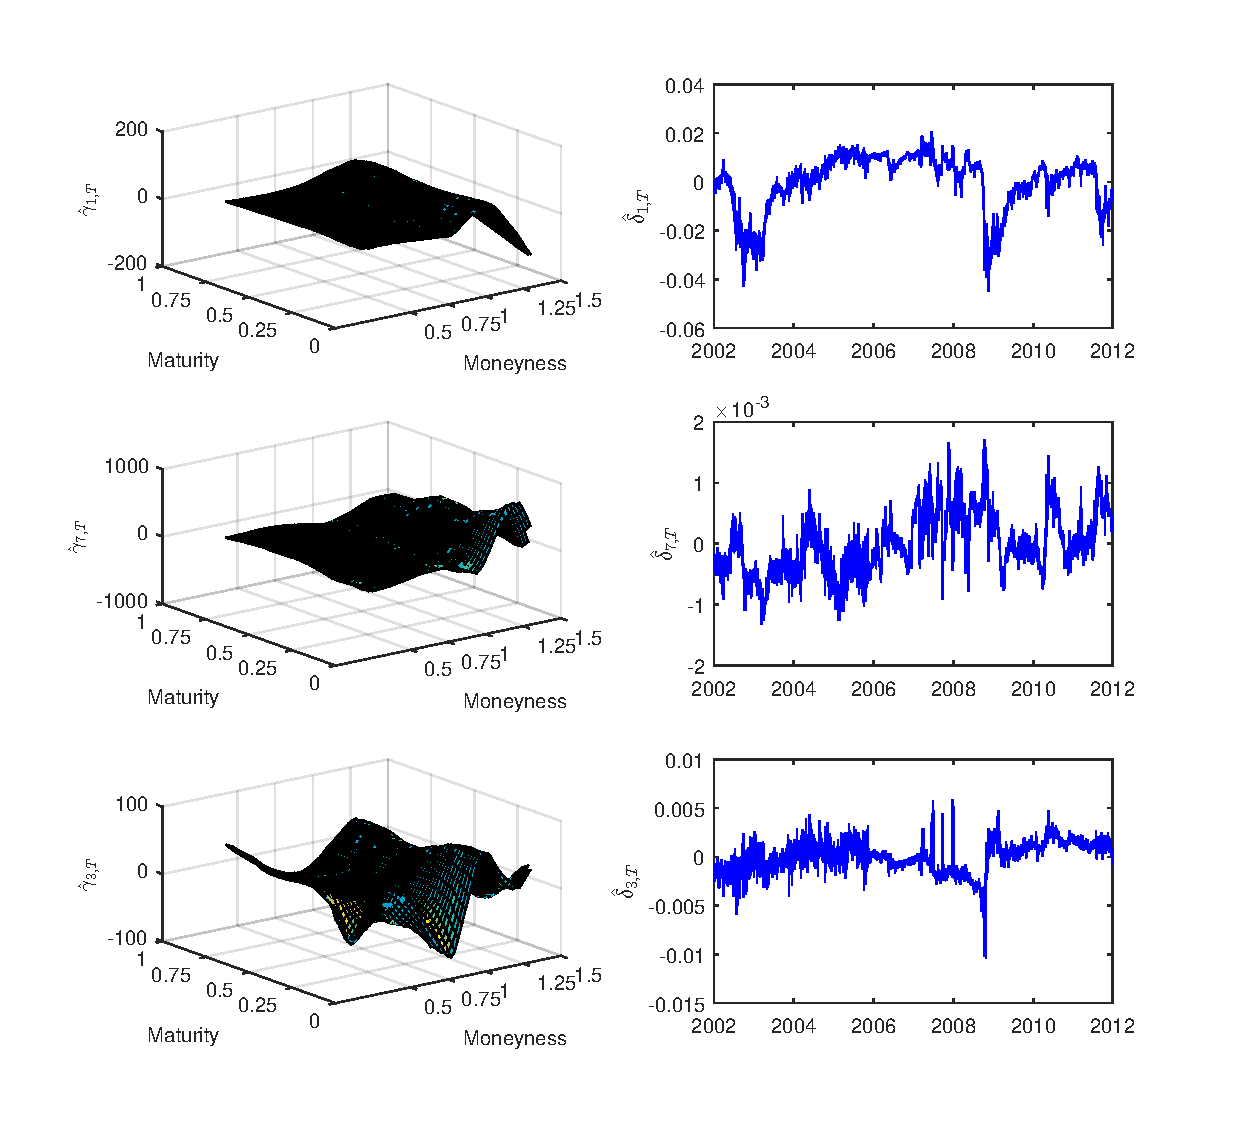
\includegraphics[width=1.0\textwidth]{figures/Nonorthogonalbasis20160521}
%\includegraphics[width=1.00\textwidth]{figures/Nonorthogonalbasis1} \\
%\includegraphics[width=1.00\textwidth]{figures/LoadingsFPCA1}
%\includegraphics[width=1.00\textwidth]{figures/Nonorthogonalbasis2} 
%\caption{\label{second_comp} Left: Call options on the expiration day. Right: Second non-orthogonal component $\hat{\gamma}_{2,T}$}
\caption{\label{nonort} Estimated non-orthogonal components and their loadings obtained by the decomposition of $\hat{M}^{(0)}$, in decreasing order of explained variance from up to bottom}
\end{center}
\end{figure}


During this period, there are not many observations available for the call prices with strikes larger than the current stock index price for small maturities. Together with the absence of a call string with close enough maturity on the following trading Monday, this introduces bias in the smooth estimated call surface, for grid values outside the range of observation points. %, stemming from the extrapolation problem for the local kernel regressions. 
However, we cannot rule out the possibility that the importance of the second component is not due to an error in pre-smoothing of the call options used for the estimation of $M^{(0)}$ because even if we recalculate the explained variance for all the components after excluding the estimated loadings from this time interval, this factor still remains the second most important. The shape of the second estimated component $\hat{\gamma}_{2,T}$, displayed in Figure \ref{exp}, suggests that it is related to the short end of the SPD term structure effect. The other components $\hat{\gamma}_{4,T}$, $\hat{\gamma}_{5,T}$, $\hat{\gamma}_{6,T}$ and $\hat{\gamma}_{8,T}$, whose loadings have similar behavior, are similar in shape to the four components we have discussed so far, i.e., $\hat{\gamma}_{1,T}$, $\hat{\gamma}_{2,T}$, $\hat{\gamma}_{3,T}$ and $\hat{\gamma}_{7,T}$. It is yet not totally clear but it is well possible that they are related to the asymmetric behavior of the option prices along the maturity direction, i.e., the term structure effect of the SPDs. %- more than one factor is necessary to explain the variation in the time to maturity direction. %We therefore focus on the remaining three components. %The evidence indicate is an indicative that the importance of the second component is due to an error in pre-smoothing of the call options used for the estimation of $M^{(0)}$, and we exclude it from our further analysis. Note that even if we recalculate the explained variances for all the components after removing the loadings from this time interval, this factor still remains important, \color{red}which may imply that the smoothing error affects the results for our entire sample \color{black}. Further, we look at the shape of the other components and the dynamics of their corresponding loadings. The loadings of components $\hat{\gamma}_{4,T}$, $\hat{\gamma}_{5,T}$ and $\hat{\gamma}_{6,T}$ suffer from the same problem as $\hat{\delta}_{2,T}$. We therefore remove them from the candidate factors. \color{red} ???? they are related to short term effects. \color{black}

%Further $\hat{\gamma}_{4,T}$ and $\hat{\gamma}_{7,T}$ are similar in shape to $\hat{\gamma}_{2,T}$ and


%We further report on the other the case $L=3$, which is an upper bound for $L_d$. We also discuss subsequently the effect of including additional factors on the stability of results. For visualization, we multiply the estimated components by the standard deviation of the corresponding loadings. 
%\begin{figure}[ht]
%\begin{center}
%\includegraphics[width=1.00\textwidth]{figures/phi6}  
%\caption{\label{ort} First six orthogonal components obtained by the decomposition of $\hat{M}^{(0)}$}
%\includegraphics[width=1.00\textwidth]{figures/phi}  
%\caption{\label{ort} First eight orthogonal components obtained by the decomposition of $\hat{M}^{(0)}$}
%\end{center}
%\end{figure}




%The other three most important estimated non-orthogonal components 
The remaining three estimated components are displayed in Figure \ref{nonort}, in order of their explained variance, see equation (\ref{varnno}). %To enable comparison, they have been multiplied by the standard deviation of the corresponding loadings. %Scaled $\hat{\gamma}_{1,T}$ and $\hat{\gamma}_{3,T}$ are similar in hight but the peak of 
%The first component is aligned with the mean, and has positive values around the peak and negative around the tails. The other two components resemble the orthogonal components in the simulation study. Some differences stem from the fact that the empirical SPD are left-skewed, compared to the right-skewed mixtures of log-normals. %This also explains a lower first 'valley' in the second component. Another difference in the tail behavior of the first two components - steep slope and negative values - might be due to interpolation errors in the regions with few observations. Other than that, the components provide a similar interpretation to those in the simulation study. 
These three components describe three types of asymmetry present in the dynamics of the SPDs. Their interpretation, is linked to the shape of the empirical mean of the SPD, which has a long tail on the left side of the peak. %A negative skew reflects the market expectation that the future stock index will be above its forward value. While negative skewness risk can bear excess returns, during periods of economic downturn, the investors prefer positively skewed distributions. 
The first component has positive values around the peak and negative around the tails and is related to the volatility dynamics. An increase in the loadings of this component decreases the volatility of SPD. The second component has a lean 'valley' at the left of the sample mean, which takes negative values, and a more pronounced 'hill' at the right, which feature positive values. This component emphasized the dynamics of negative skewness and induces as well changes in the kurtosis of the density. % mass around the mean of the distribution and can 
We interpret it as the negative skewness factor. The third component has a more symmetric 'valley-hill' pattern, which shifts mass around the central region of the density. It also influences the density far left tail. A positive shock in the direction of this components increases the negative skewness, while a large enough negative shock will render the SPD positively skew. This component is interpreted as the sign of skewness factor.  % and influences also particularly the the to the tails at the expense of the regions in between in a disproportionate fashion. The variations are larger in amplitude in the left half of the distribution. This component is interpreted as a kurtosis factor. 
%crosses zero four times (for fix maturity). It influences the kurtosis of the density: it %simulated that of the second component is shifted to the right and is steeper for maturities of less than three months - options with shorter maturities are supposed to react stronger to changes. Both their right tails are negative, possibly due to the smoothing errors outside the observable data region. 


%The loadings $\hat{\delta}_{1,T}$, $\hat{\delta}_{7,T}$  and $\hat{\delta}_{3,T}$ display a time-varying volatility regime, which divide the sample in three sub-periods that may reflect the impact of the global environment on the option prices. The end of 2005 marks the decline in the global liquidity and the end of 2008 is the conjectured conclusion of the global financial crises. Formal statistical tests for the equality of the loadings variance within the three subperiods can be run for a more thorough analysis. This can possibly unveil interesting economic questions, which will have to be left for further research. %We do not follow up on these observations because, as we show in the following, this variation is not longer present after orthogonalizing the loadings. %  \color{red}Changes in the mixture's distribution? We can interpret these as possibly changes in the mean function of the call prices or changes in the underlaying components Irina cite paper\color{black}. We will look at this issue in our following analysis. We will briefly return to them when discussing the connection between the SPDs and VDAX, in section \ref{?}. 
%Therefore, we delete components two and four to represent the dynamics of $\bar{C}^{((2,0))}$ in terms of the orthogonal components, see figure \ref{rez}. 


%From the simulation study we know that the variation explained by the third orthogonal component for density mixtures is significantly smaller than those of the first two. This is likely to translate in relatively small variations of the call prices as well. However, this component is important for explaining the moments of the DAX returns, for hedging or pricing purposes. We are therefore interested to identify it from the noisy data. Based on the criteria for the choice of number of factors, a less conservative choice for a proper truncation of the model is $L=9$. 

% If we exclude this period from our sample the forth component is not 'loosing' its importance as well.
 %Here, it proves useful to have some prior knowledge about the shape of the components we expect to identify empirically.
%When investigating the variation of densities, one must be cautions because - as seem in the simulation study - the variation explained by further components is relatively small compared to the first two ones. Hence, without a proper ``shape marker/identifier'' one might easily confound them with noise. 
 %It proved useful to have some prior knowledge about the shape of the orthogonal components in order to choose a proper truncation of the model. 
%First, we look at the shape of the components and the dynamics of their corresponding loadings. Components $\hat{\gamma}_{4,T}$ and $\hat{\gamma}_{7,T}$ are similar in shape to $\hat{\gamma}_{2,T}$ and their loadings suffer from the same problem as $\hat{\delta}_{2,T}$. We therefore remove them from the candidate factors.

%\begin{figure}[ht]
%\begin{center}
%\includegraphics[width=1.00\textwidth]{figures/Rotatedorthogonal1} \\
%\includegraphics[width=1.00\textwidth]{figures/Rotatedorthogonal2} 
%\includegraphics[width=1.00\textwidth]{figures/Orthogonalbasis1mew}\\
%\includegraphics[width=1.00\textwidth]{figures/Orthogonalbasis2mew}
%\caption{\label{second_comp} Left: Call options on the expiration day. Right: Second non-orthogonal component $\hat{\gamma}_{2,T}$}
%\caption{\label{nonortrot} First four rotated orthogonal components when including  $\hat{\gamma}_{1,T}$, $\hat{\gamma}_{2,T}$ and$\hat{\gamma}_{3,T}$}
%\end{center}
%\end{figure}

% The purely autoregressive model explains the dynamics of the risk-neutral implied moments rather well. \color{red} Adding exogenous variables to the vector autoregression does not improve the explanatory power of our model. \color{black} 
 
 
 

%One-step ahead forecasting accuracy, measured as the RMSE of the in-sample forecasting errors imply that the first model is better in terms of prediction. These models can be used to investigate Granger causality relations between the loadings. 



%The shape features of the three components from Figure (\ref{nonort}) and their ordering according to the explained variance are stable to orthogonalization, when we use the truncation choice  $\sum_{r\in \{1,3,7\}}\hat{\delta}_{r,T}\hat{\gamma}_{r,T}$. 
The functional principal components for the reduced model $\sum_{r\in \{1,3,7\}}\hat{\delta}_{r,T}\hat{\gamma}_{r,T}$ resemble closely the three components from Figure \ref{nonort}. % is possibly introduced through the dynamics of the interest rate term structure
%This means that if we ignore the term effect, which expresses the asymmetric reaction intensity to changes in the economic environment between the short and long term term option prices, the first three orthogonal components of the reduced model can still be interpreted as volatility, skewness and kurtosis factors. To avoid the burden of introducing additional notation we use non-orthogonal estimates in our further analysis. 
Further analysis shows that if we add any of the term structure components, whose loading feature a behavior similar to $\hat{\delta}_{2,T}$, with their inherent jump before, the shape of the components changes slightly. In addition, the loadings of all orthogonalized components are 'contaminated' with jumps. %Therefore, we use only three basis to describe the dynamics of SPDs % if the term structure effect of the SPDs is not considered. Variations of SPD in the maturity dimension introduces additional components, which are required to describe the asymmetric SPD changes for short and long maturities, similarly to the main modes of variation in the reduced model. %to reflect the uneven changes introduced by the term structure variation. %around the mean, skewness and kurtosis.
In fact, all the loadings of the estimated components (not displayed here) by decomposing $\hat{M}^{(d)}$, for $d=(2,0)$ display the jump-behavior we described before between mid-February 2007 and mid-September 2008. In that sense, the previous approach seems to provide more accurate estimates that allow for a better interpretation of the results.
%We verified this by varying the number of factors before orthogonalization. We found that the shape features of the first three orthogonalized components from is preserved, while their loadings display jumps, similarly to $\hat{\delta}^{(d)}_{2,T}$ if any of the other 'noisy' components are added, similarly to the loadings $\hat{\delta}^{(d)}_{r,T}$. In fact, shape-wise $\hat{\gamma}_{1,T}$, $\hat{\gamma}_{2,T}$ and$\hat{\gamma}_{3,T}$ correspond to the estimates $\hat{\varphi}_1^{(d)$, $\hat{\varphi}_2^{(d)$ and $\hat{\varphi}_1^{(d)$. The other three orthogonal basis obtained from the decomposition of $\hat{M}^{(d)}$, are also related to the behavior of short term maturities. For instance, $\hat{\gamma}_2^{(d)$, closely resemble $\hat{\varphi}_4^{(d)$. We posit that three basis are necessary to explain variation of the SPDs if the term effect is not considered. The term effect introduces additional components, that decompose the term variation in variation around the mean, skewness and kurtosis. %The correlation structure between the loadings $\hat{\delta}_{r,T}$ and $\hat{\delta}^{(d)}_{r,T}$ are showed in table \ref{????}.

%Further, we analyze our results in terms of the orthogonal components. This allows us to perform a direct comparison between the estimation of the SPD by the two methods we presented in the previous sections. %compare them with the alternative estimation method based on the decomposition of $\hat{M}^{(d)}$. 
%For this, we rotate the remaining six components, by applying a projection $a$, such that: $\sum_{r\in \{1,3,5,6,8,9\}}\hat{\delta}_{r,T}\hat{\gamma}_{r,T}=\sum_{r=1}^6a_r \tilde{\varphi}_r^{(d)}$, where $\tilde{\varphi}_r$ are the functional principal
%components for the reduced model and $a_r$ the corresponding loadings. By proceeding in  this way, the important commonalities in the nonorthogonal factors will be concentrated in even fewer components. %This also allows us to interpret our results in terms of components with known shape and also compare them with the alternative estimation method based on the decomposition of $\hat{M}^{(d)}$. 
%The results are displayed in figure \ref{nonortrot}, for the first four orthogonalized components. The first three closely resemble the orthogonal components from our simulation study. One difference stems from the fact that the empirical SPD are left-skewed, compared to the right-skewed log-normals and their mixtures. This also explains a lower first 'valley' in the second component. Another difference in the tail behavior of the first two components - steep slope and negative values - might be due to interpolation errors in the regions with few observations. Other than that, the components provide a similar interpretation to those in the simulation study. They describe three type of asymmetries present in the dynamics of the SPDs. The first component that peaks at the same location as the mean curve, redistributes mass from the peak to the tails and can be related to the volatility dynamics. The second component, can be interpreted as influencing the skewness of the density: it adds mass to the central region and subtracts mass from the tails. The third component, shifts the density mass between the left and right sides and can be linked to the skewness factor. The corresponding loadings $a_r$ are no longer appear to be heteroskedastic. We will return to the analysis of their dynamics in the next subsection. (short characterization of the dynamics that anticipate findings in the next section).


%Two orthonormal components explain almost the entire variance of the reduced model, namely $99.74\%$ and $0.26\%$ respectively. 3rd??? The role played by the two components in explaining the variation of the SPD must be interpreted with caution, as changes in different regions of the underlying density may signal changes in the characteristics of underlying economic risks and market reaction to them, as well as impact the prices of the contingent clams on the underlying asset in a disproportionate fashion. For instance, it is well known that the deformation of the tail distribution conveys important information about the probability of extreme events that affect portfolio performance and hedging decisions. For the European options, small changes in the small probabilities can affect substantially the prices of far out of the money (OTM) options. Our further ananlysis suggests that both components are essential in undertanding the dynamics of SPD. Pricing of OTM Puts and Calls - asymmetris in the 

%The second orthonormal component presents a positive peak situated around the peak of the mean. The right tail displays more negative values whereas the values of the component in the left tail fluctuate around zero negative. A positive shock in the direction of this component increases the peakness of SDP over the mean and decreases the mass of the distribution in the tails, in particular in the right one. 

%\color{red}How do the factors influence the option prices?\color{black} Changes in the shape of the SPD translate to changes in the option prices. Whenever the probability mass for certain values of moneyness increases it will result in higher weights associated to the payoffs of the option in that particular states. For instance, a positive shock in both components will result in more expensive medium range OTM and cheaper far OTM calls. Conversely, a negative shock will make the prices of both far OTM put and call options increase while the prices of medium range OTM calls will decrease. This behavior can be related to the hedging behavior on the option market, see the discussions in \cite{Bollen:04}, \cite{Constantinides:11} and \cite{Kra:15}. % explain this behavior by  they don't like uncertainty. 



%that including additional components preservesthe explained variance increases with each with each component that we include in the reduced model.


%We verified the consistence of our results by varying the number of factors before orthogonalization. We started by including only two components, $\hat{\gamma}_{1,T}$ and $\hat{\gamma}_{3,T}$, and investigated the principal components and their loadings for the reduced model. We repeated the procedure by increasing the number of components one at a time. We found that including additional components preserves the features of the first two orthogonalized components from figure \ref{nonortrot}, while the explained variance increases with each with each component that we include in the reduced model. The shape of the third component becomes stable once we add $\hat{\gamma}_{6,T}$. If we include only three components ($\hat{\gamma}_{5,T}$) then the third principal component is similar in shape to the fourth component in figure \ref{nonortrot}. Finally, deciding how large $L_d$ should be taken in practice, i.e. how many principal components, is both a matter of interpretation ability in terms of the shape of the components and of their loadings to capture as much variance in the data as possible, and adequately describe the dynamics of the underlying high-dimensional curves by correctly eliminating the noise terms.  \color{red} approximate factor model ???\color{black}



%The loadings are strongly correlated. This means that a factor model may be appropriate.
%This observation is supported by the results from the decomposition of $\hat{M}^{(d)}$, for $d=(2,0)$. Most of the criteria for choosing $L_d$ by this approach suggest six components. 

%The optimal choice for $L_d$ from the $CP^{(d)}$ criteria gives at least six components, while both the eigenvalue ratio and $IC^{(d)}$ give six components. If we look at Figure \ref{ort}, we notice that there are three pairs of similarly-shaped components: the first pair $\hat{\varphi}^{(d)}_{1,T}$ and $\hat{\varphi}^{(d)}_{2,T}$ relate mainly to changes in the volatility, the second pair $\hat{\varphi}^{(d)}_{3,T}$ and $\hat{\varphi}^{(d)}_{5,T}$ looks similar to $\hat{\gamma}^{(d)}_{2,T}$, while the third pair $\hat{\varphi}^{(d)}_{4,T}$ and $\hat{\varphi}^{(d)}_{6,T}$ is similarly shaped to the negative skewness component from the previous decomposition. %The first pair relate to the volatility, the second pair appear similar to $\hat{\gamma}^{(d)}_{2,T}$, while the third pair is similar to the negative skewness factor. %However, this interpretation is not straight-forward and investigating additional components might shed additional light into this issue. 


%We plot as well $\hat{\varphi}^{(d)}_{7,T}$ and $\hat{\varphi}^{(d)}_{8,T}$, which can be interpreted as skewness sign factors. These components are quite small and some of the criteria for the selection of the number of factors based on this approach might be overlooking his importance. Except for the first components estimated by each method, the loadings corresponding to $\hat{\varphi}^{(d)}$ and $\hat{\gamma}^{(d)}$ display only mild or low correlations. Therefore, a direct correspondence between the components is not straight forward. However, an approximate factor model is possible to hold for these data. As regards the 'duplicity' of the components, our results are most likely a manifestation of the SPD term effect, e.g. options with various maturities react differently to changes in the economic conditions. Accordingly, two factors in the term structure dynamics imply that two sets of components are required to explain the SPD implied expectations of long and short-run moments. This assumption is supported by looking particularly at the shape of the first pair, where the first component is relatively flat and describes reactions in the SPDs for longer horizons and the second component is steeper and describes reactions in the SPDs for short maturities.%.  we contend that the two sets of components describe reactions in the SPDs for long and short maturities. %as clear as in the case of $\hat{\gamma}^{(d)}_{r,T}$s.  
%Not displayed here, all the loadings of the estimated components by decomposing $\hat{M}^{(d)}$ display the jump-behavior we described before between mid-February 2007 and mid-September 2008. In that sense, the previous approach seems to provide more accurate estimates that allow for a better interpretation of the results. %These results occur because the extrapolating error is worse for the second derivative. They are, however, stable in terms of the volatility of the loadings. 
%Approximate factor model might be possible if we look at figure \ref{ort}.

%The estimated correlations between $\hat{\delta}_{r,T}$ and $\hat{\delta}^{(d)}_{r,T}$ displayed in table \ref{corrt} show a strong correlation only between the loadings of the first components estimated by each method, while the other correlations are quite small. No significant correlations are obtained after applying FPCA to the reduced model either. (Try 8 components). The results are thus mixed, if a factor model is appropriate for our data. (Maximum correlation - maximize correlation between projections - Markus paper).

%From the simulation, we have learned that the variance explained by each additional components decreases 'more than' exponentially for each additional factor added, when there is no term structure effect. This is why, when decomposing the variance explained ... 1.2550     0.0025      0.0001 multiplied by a factor of $10^7$. In Table 2 - Reordered variance. How to decide on the number of factors? 


%The optimal choice for $L_d$ from the $CP^{(d)}$ criteria gives $L_{\max}$ components for $L_{\max} \leq 5$, while $IC^{(d)}$ gives six components. The forth component is obviously related to the short-term maturity effect. In general, the loadings of all estimated components by decomposing $M^{(d)}$ display the jump-behavior we described before between mid-February 2007 and mid-September 2008. These results occur because the extrapolating error is worse for the second derivative.They are, however, stable in terms of the volatility of the loadings. 

% for the dynamics of state price density surfaces.
%The first two estimated principal components are similar to the functional principal components of the reduced model, see figure \ref{ort}. The pairwise correlation between their corresponding loadings is also high, $corr(\hat{\delta}^{(d)}_{1,T},a_1)=0.75$ and $corr(\hat{\delta}^{(d)}_{2,T}a_2)=0.73$. The third component does not offer conclusive evidence either with respect to the shape or the correlation $corr(\hat{\delta}^{(d)}_{1,T},a_1)=-0.23$, which is relatively small. The forth component is obviously related to the short-term maturity effect. In general, the loadings of all estimated components by decomposing $M^{(d)}$ display the jump-behavior we described before between mid-February 2007 and mid-September 2008. %Further components are also relatively smooth compared to $\tilde{\phi}_4^{(d)}$ and they seem also affected by the small-maturities effect. 
%These results occur because the extrapolating error is worse for the second derivative. % it might be that the second derivative amplifies the noise. One problem that occurs when taking derivatives is 
%They are, however, stable in terms of the volatility of the loadings. 
%A factor model with two components based on equation 
%we choose the number of factors to be = to the largest variance before the reordering 

 \begin{figure}[ht]
\begin{center}
\includegraphics[width=1.00\textwidth]{figures/ACPAC}  
\caption{\label{acpac} Autocorrelation (AC) and partial autocorrelation (PAC) of the estimated loadings and of their difference}
\end{center}
\end{figure}

\subsubsection{Dynamic analysis of the loadings }
We look at the dynamics of the SPD as summarized by the reduced model. By construction, the loadings are orthogonal, however their movements suggest strong dependencie. A negative skewness of the SPD reflects the market expectation that the future stock index will be above its forward value. Usually, the negative skew increases together with the implied volatility. While negative skewness risk can bear excess returns, during periods of economic downturn, the investors prefer positively skewed distributions. This can be seen when looking at the large negative values of $\hat{\delta}_{3,T}$ which, in effect, shift the SPD mass from the positive to the negative side of the distribution, in conformity with an increase in the risk aversion of investors.

In the following, we would like to understand how past realizations of the loadings influence present observations. 
%How past values of Ds influence future values. 
Figure \ref{acpac} displays the sample autocorrelation and partial autocorrelation
functions for the loadings from Figure \ref{nonort} and their first difference. Autocorrelation functions of the loadings decay very slowly suggesting nonstationarity in the time series. Standard tests for the presence of unit roots are performed for the loadings provide evidence of unit-root in the level of the loadings. Engle-Granger and Johansen tests for pairwise and multiple cointegration relationship between the loadings indicate that the series are cointegrated.


After taking the first difference the high persistence vanishes and there is a single significant spike for the first lag.
The partial autocorrelation functions for the first difference spike at the first lag and decreases over the next few lags.
%slowly for the next three-four lags. 
The results suggest that an ARIMA(1,1,1) %or ARIMA(4,1,1)
model might be appropriate to model the loadings. Its continuous-time equivalent, the mean-reversion process, has been used to model the changes in the implied volatility surfaces, see \cite{Cont:02}. In the following, we focus on the discrete time model and use a vector-autoregressive model (VAR) for the first difference of the loadings. 
\[
y_i=\Omega y_{i-1}+\varepsilon^{\footnotesize{VAR}}_i,
\]
where $y_i=(\Delta \hat{\delta}_{i1} \mbox{ } \Delta \hat{\delta}_{i3} \mbox{ } \Delta \hat{\delta}_{i7})^{\top}$, for $\Delta \hat{\delta}_{ir} =(\hat{\delta}_{ir,T}-\hat{\delta}_{i-1 r,T})$, and $\Omega$ is a coefficient matrix. The results of the estimation procedure are presented in Table \ref{tab1}. This model specification also allows us to employ a Granger causality test to assess whether the loadings of one component is actually useful in predicting the future levels of the other SPD components. The results of the test, summarized in Table \ref{tab2} show that daily changes in the negative skewness factor are not caused by the changes in the volatility factor. The other variables Granger-cause each other. \color{red}Also notice that we have tested for Granger Causality for multiple lags and the results are quite robust. \color{black}%\color{red}loadings are integrated. Also verify this for different Lag size - up to three months: Need to redo it but it seems that d3 cannot be predicted. also, from one to four weeks it can be predicted.  \color{black}


\begin{table}\label{granga}
\footnotesize 
\begin{center}
%\begin{center}
\begin{subtable}{.5\linewidth}
\begin{tabular}[t]{c|c|c|c|c}
\hline \hline
\footnotesize $\Omega_{i,j}$ & $j=1$ & $j=2$ & $j=3$& a. $R^2$\\
\hline
\footnotesize $i=1$ &    $-8.84^{**}$    & $58.59^{***}$   &  $91.05^{**} $  &  0.1328\\
\footnotesize $i=2$  & $ 3.96^{**} $  & $-32.90^{***}$   &$ -35.58^{**} $ &  0.2012\\
\footnotesize $i=3$ &   $0.22$ &  $-2.51^{***} $  & $-28.90^{***}$  & 0.1589 \\
%\hline
%a. $R^2$ &  0.1328 &  0.2012 & 0.1589 \\
\hline \hline
\end{tabular} 
     \caption{\label{tab1} \footnotesize VAR coefficient matrix}
     \end{subtable}
     %\end{center}
 \begin{subtable}{.5\linewidth}
\begin{tabular}[t]{c|c|c|c}
\hline \hline
%$H_0:$
\footnotesize  $j \not \rightarrow i $ & $j=1$ & $j=2$ & $j=3$\\
\hline
\footnotesize $i=1$ &    $3.78^{*} $  & $65.58^{***} $  & $10.63^{***}$ \\
\footnotesize $i=2$  &  $4.37^{**} $  & $89.19^{***} $   & $8.77^{***} $ \\
\footnotesize $i=3$ &  $ 1.10$ &  $24.67^{***}$ & $125.41^{***}$  \\
\hline
%$H_0:$
\footnotesize  $ j\neq i \not \rightarrow i $  &  $82.84^{***} $&  $26.30^{***} $ & $49.35^{***}  $\\
\hline \hline
\end{tabular}
 \caption{\label{tab2} \footnotesize Granger test statistics}
 \end{subtable}
  \caption{Estimation and test results for the VAR(1) model of the first difference for loadings $\hat{\delta}_{1,T}$, $\hat{\delta}_{3,T}$, and $\hat{\delta}_{7,T}$. The reported coefficients are multiplied by $10^2$. Granger causality testing that $y_i$ is not caused by $y_j$ (or any $y_j$, $j\neq i$) uses a variance-covariance matrix estimated under the assumption of heteroskedastic and correlated covariance of the errors. $^{***}p<0.01, ^{**}p<0.05, ^{*}p<0.1$}
  \end{center}
\end{table}


All variables react negatively to changes in their own past levels. Previous increases in the negative skewness and kurtosis via $\hat{\delta}_{3}$ and $\hat{\delta}_{7}$, lead to higher $\hat{\delta}_{1}$ (lower implied volatility) in the future. Past values of $\hat{\delta}_{3}$ and $\hat{\delta}_{7}$ have negative effects on each other. Increases in the volatility factor $\hat{\delta}_{1}$ (lower implied volatility) predicts higher $\hat{\delta}_{3}$ the next trading day. However, these predictions are at the level of the entire sample. The relatively low values for the $R^2$ in Table \ref{tab1} can be partly explained by looking at the dynamic contemporaneous correlation structure for the first-difference of loadings. The graph might be an indicative that for forecasting purposes, one is advised to use a time varying VAR model. 


\begin{figure}
\begin{center}
\includegraphics[width=1.00\textwidth]{figures/corr_load}  
\caption{\label{window}  100-days moving window correlation coefficient for the first-difference of the loadings and volatility of implied volatility}
\end{center}
\end{figure}

Examining closer the dynamic relation for the loadings first difference, represented in Figure \ref{window} through the 100-days moving window correlation coefficient, we see that for most of the times the volatility and negative skewness factors move together. 
%oftentimes the above mentioned correlation is close to -1  and but its strength also weakens and is sometimes reversed. 
%The correlation structures that involve $\hat{\delta}_{7,T}$  show that this component expresses reactions to sudden and shorter term changes in volatility. 
Oftentimes the correlation of their difference $corr=(\Delta \hat{\delta}_{i1} , \Delta \hat{\delta}_{i7})$ is close to $-1$ and its strength weakens and is sometimes reversed, in a strong connection to the movements of the volatility of implied volatility ($Vol_{IV}$), computed as a 100-days moving window standard deviation of the daily implied volatility index. %Its correlation with delta d1 is negative for most of the time, except in 2009 when after a sudden increase and subsequent decrease in volatility d7 continue to decrease and become negative. This reverse reaction means that the OTM put options become more expensive as volatility increases.  
The reversion in the correlation sign following the financial crises means that the OTM put options become more expensive as volatility increases. This phenomenon is explained in the empirical financial literature through the net buying pressure of index options (\cite{Bollen2004}, \cite{Garleanu2009}). Overall, $\hat{\delta}_{7,T}$ is linked to sudden and short-term changes in volatility.


%A similar behavior can be induced by $\hat{\delta}_{3,T}$. From 2006 to the end of 2008, $\hat{\delta}_{3,T}$ decreases and becomes negative during the financial crisis. 
After sustained periods of increases in the implied volatility, particularly between 2006 to the end of 2008, $\hat{\delta}_{3,T}$ decreases substantially, giving rise to more expensive OTM puts and relatively cheaper deep OTM options. 
%This increase in the negative skewness  (and/or or less fat left tail) 
The overall flattening of the left tail together with volatility increases is a manifestation of the implied volatility skew puzzle, as documented by \cite{Constantinides2015}. The authors explain it through the reduction in supply of put options from credit-constrained market makers when the demand for puts increases. Our findings according to which the difference between the prices of OTM and ATM put options decreases during the financial crisis, is consistent with their observation that the implied volatility skew declines.

% implied volatility skew puzzle is that the difference between OTM
%d 7 ---- component expresses reactions to sudden and shorter term changes in volatility. 

%The evidence shows that d3 and d7 can be seen as long and respectively short term reaction to changes in volatility and volatility of volatility. 


%The VAR coefficients imply that negative shifts in the first component, consistent with an increase in implied volatility, or decrease in the negative skewness, through negative movement of $\hat{\delta}_{7}$. A decrease in the negative skewness, through negative movement of $\hat{\delta}_{7}$. In effect, the slope of the left side of the SPD decreases and the price of deep out-of-the-money (OTM) puts increases.
%For not too small moneyness levels, this means less probability mass in the left side of the SPD, which translate in cheaper out-of-the-money (OTM) puts. For deep OTM puts, positive movements of $\hat{\delta}_{i3}$ imply a fatter left tail and hence higher prices. 
 



\subsubsection{Relationship to the dynamics of VDAX index } %Standard tests for the presence of unit roots are performed for both loadings and their first difference: Augmented Dickey-Fuller (ADF), Kwiatkowski, Phillips, Schmidt, and Shin (KPSS), Phillips-Perron for one unit root(PP) and the Variance ratio test for random walk (VR), all provide evidence of unit-root nonstationarity in all the loadings of the first seven components $\hat{\gamma}_{r,T}$. 
% available from Deutsche B{\"o}rse AG. 
The VDAX index expresses the implied volatility of the DAX recovered from the prices of call and put options. It is an important indicator on the market, often called ``fear'' index because it reflects the market expectation for the 30 day ahead volatility of the DAX index under the risk neutral measure, which is then annualized. %VDAX represents the theoretical price of one-month variance swaps on the DAX index.
%that gives a synthetic value for the implied volatility (IV) surface. 
%the connection between the characteristics of options and the VDAX index requires the transformation of option prices in the equivalent implied volatilities.
%Until the end of 2006, it is computed from the intraday ATM and afterwards it uses in addition the OTM DAX call and puts options with varying maturities. 
A volatility sub-index is calculated for each traded maturity and the volatility index itself is calculated via an interpolation of the two sub-indexes closest to the 30 days expiration. % between one month and two years. 
%Deutsche B{\"o}rse AG provides a detailed methodology for its calculation. % can be found at \hyperref{http://deutsche-boerse.com/}.
%The dynamic of the index is shown in Figure \ref{???}. 
As an indicator of the second moment of the DAX index under the SPD, we investigate how well the loadings explain its dynamics. %the dynamics of the daily VDAX index. 



 \begin{table}[ht] 
 \footnotesize 
\begin{center}
\begin{tabular}{c|r@{.}l  r@{.}l  r@{.}l  r@{.}l  r@{.}l  r@{.}l  r@{.}l  r@{.}l}\hline\hline    
d.v.&\multicolumn{2}{c}{$\hat{\delta}_{1,T}$}&\multicolumn{2}{c}{$\hat{\delta}_{2,T}$}&\multicolumn{2}{c}{$\hat{\delta}_{3,T}$}&\multicolumn{2}{c}{$\hat{\delta}_{4,T}$}&\multicolumn{2}{c}{$\hat{\delta}_{5,T}$}&\multicolumn{2}{c}{$\hat{\delta}_{6,T}$}&\multicolumn{2}{c}{$\hat{\delta}_{7,T}$}&\multicolumn{2}{c}{Adj. R$^2$ }\\ \hline
% $VDAX$    & 0&9428&   -0&1531& 0&1420 & 0&0130&  0&0652&  0&0033 &  -0&1172& 0&977\\ %0&0221&  
% \small{VDAX}    & 0&9221&   -0&1362& 0&1458 & 0&0146&  0&0411&  0&0109 &  -0&0965& 0&975\\ %0&0221&  
% \small{VDAX}    & 0&9374&   \multicolumn{2}{c}{-}& 0&1787 & \multicolumn{2}{c}{-}&  \multicolumn{2}{c}{-}&  \multicolumn{2}{c}{-} &  -0&0935& 0&972\\ 
\footnotesize  \small{VDAX}    & -0&9221&   0&1362& -0&1458 & -0&0146&  -0&0411&  -0&0109 &  0&0965& 0&975\\ %0&0221&  
\footnotesize  \small{VDAX}    & -0&9374&   \multicolumn{2}{c}{-}& -0&1787 & \multicolumn{2}{c}{-}&  \multicolumn{2}{c}{-}&  \multicolumn{2}{c}{-} &  0&0935& 0&972\\ 
 %\hline
 %\small{DAX} & -0&5566&    -0&1268&     -0&0373&     -0&1167&     -0&0730&     0&1811&   -0&5258& 0&646\\ 
 %\small{DAX}    & 0&5464&   \multicolumn{2}{c}{-}& 0&0385 & \multicolumn{2}{c}{-}&  \multicolumn{2}{c}{-}&  \multicolumn{2}{c}{-} &  -0&5372& 0&571\\  %  $VDAX$    & 0&9428$^{***}$&   -0&1531$^{***}$ & 0&1420$^{***}$ & 0&0130&  0&0652$^{***}$&  0&0033$^{***}$ &  -0&1172$^{***}$ & 0&977\\ %0&0221&  
% $DAX$ & -0&5566$^{***}$&    -0&1268$^{***}$&     -0&0373$^{***}$&     -0&1167$^{***}$&     -0&0730$^{***}$&     0&1811$^{***}$&   -0&5258$^{***}$& 0&646\\
    \hline\hline
    \end{tabular}
    \caption{\label{dax} Contemporaneous regressions of the VDAX index on the loadings of $\hat{\gamma}_{r,T}$. All coefficients are significant at 99\%. confidence level}
\end{center}
\end{table}

Statistical tests for stationarity suggest a unit root process. Cointegration tests indicate that the VDAX index and the loading series are cointegrated with high probability. This means that there is a contemporaneous relationship between them and we can express VDAX in terms of the loadings. 
%We performed pairwise and multiple cointegration relationship tests (Engle-Granger and Johansen) between the loadings and VDAX index, which indicate that all the series are cointegrated. In the following, we estimate the cointegration relationship between VDAX on one hand and the loadings on another hand.%They pairwise cointegration is not rejected for any pairs except those that include DAX. (Multivariate cointegration test.) 
%The results are reported in table XXX for the entire sample and sub-periods. They are cointegrated. VDAX - the loadings are cointegrated with VDAX for all non-orthogonal, orthogonalized, orthogonal???
%DAX??? returns
%VDAX and loadings are cointegrated and we estimate the cointegration relationship. 
%The results show that our methodology allows a simple mapping between the volatility index and the option prices. The 
%VDAX index can be understood to summarize the properties of the entire call price surface. We use a low-dimensional factor in terms of loadings, which correspond to interpretable components of the call derivative function and perform simple linear regressions of the VDAX on the loadings of the non-orthogonal components. 
The results of the linear regressions of the VDAX on the loadings of $\hat{\gamma}_{5,T}$ components are reported in Table \ref{dax}, for three and seven component loadings. The most important factor for explaining the dynamic of VDAX is $\hat{\gamma}_{1,T}$. %This can be also see looking at the time series of its loadings and VDAX. 
Both changes in the skewness and kurtosis improve the fit but their impact is decidedly much smaller. Variances increases are associated with to negative movements of these components, which results in flatter densities.  
In the first regression, the coefficient of $\hat{\delta}_{2,T}$ seems to be relatively important but if we compare the smaller nested model, we see that the impact of the other four loadings improve the overall fitness very little. %Moment matching argument to VDAX suggest that the projection of loadings on the space span better explains VDAX. VDAX uses a weighting information scheme for the option data available. A model selection technique suggests to choose components 1,3,5, and 8 and then the first two orthogonal components will explain over 97.00\% of the total variance of VDAX. 
%Contemporaneous correlation between the loadings and VDAX as well as the the results of regressing VDAX on the loadings are displayed in tables \ref{???}. daily regression error - 
%The methodology used to compute VDAX involves a weighted average of daily variances derived from the option prices for a fixed maturity, referred to as the nearest maturity for the desired 30 days time horizon. This methodology uses partial information available in the call prices to define an index at a unique maturity, a property that makes it difficult to replicate. Moreover, 
%a compromise between the available information and the index definition. 
Also, notice that $\hat{\gamma}_{3,T}$ is the second most important components for explaining VDAX. This shows that, even the amount of variance explained by it is very small compared to the first two ones, its importance for characterizing the moments of SPD is quite significant. Part of the reason is that VDAX is very sensitive to the changes in the tails of the SPD. %\textbf{Order of magnitude of over $10^4$.} The R$^2$ from regressing VDAX on the second loading is 0.85. The reason is that the VDAX is very sensitive to the changes in the tails of the SPD. The connection between the loadings of the first component and the VDAX more modest, R$^2$=0.54. The two manage to reproduce the dynamic of VDAX closely, as a high R$^2$=0.93 indicates. Component of the volatility that is related to changes in volatility .... then mean location ... then skewness. Show it!

%The amount of variance of the second derivative explained by the second component is very small compared to the first one. Its importance for option pricing and for the characterization of the implied volatility is however significant, as it explains a large part of the variation in the VDAX index. The coefficient of determination (cod) from regressing VDAX of the second loading is 0.85. The connection between the loadings of the first component and the VDAX more modest, cod=0.54. The two manage to reproduce the dynamic of VDAX closely, measured by the R-squared=0.93. 

%The results illustrate that we can characterize the link between the shape of the implied SPD and the volatility index in a linear fashion. %Interestingly, even if we use all the options with maturities between one week and one year that are daily available this does not add much noise to the regression of volatility for a fixed maturity. 
These results help improve our understanding of the volatility index in terms of the shape components of the SPD surface. Furthermore, if we can estimate the loadings of the factors on a particular day, we can calculate the implied VDAX quite well. %Intricated computation methd
We have investigated if the loadings have a better predictive power for the VDAX than a univariate random walk. Results, not reported here, show that even they predict VDAX fairly well, they are not superior to a random walk for VDAX. However, the forecasting model where the predictors are past loadings is still useful to model expected short-term changes in the SPD surfaces. 
 

 
 
 

%\textbf{They are not integrated: Apply difference.} For the DAX index, the other components are important, it seems. Does maybe a rotation of the loadings (obtained by maximizing variance) almost replicate the DAX index? Probably not. ??? BUT Today's expected volatility is neg correlated with the current value of the DAX index - Leverage effect(all coeff are negative). Expected skewness is negatively related (high index today - negative skewness tomorrow)- ??? weird. Kurtosis (high index today - decrease in Kurtosis tomorrow). But gamma2 could be related to the variation in the horizontal direction - 1. redo the contemporaneous regression. 2. check the forecast. 3. look at the DAX value on those days!!!! 4. Was there any short term reaction???? 5. Look at the students's presentation on VDAX surfaces. 
 
%We have repeated our estimation for different grid and the results are consistent. 






 

%We report the results for the projections of $\hat{\gamma}_{r,T}$ to orthonormal components, %$r=1,\ldots,4$ as well as the orthonormal modes of variation implied  derived by applying the FPCA decomposition to a reduced spatial representation of the derivatives, see (\ref{approx12}), with up to four components. 

 

%The shape of the orthonormal components is relatively stable when we vary the number of factors and their impact on the shape of the SPD easier to interpret. %In the following, we report the results for the case of two factors. We first refer to the figure (\ref{basis}). The empirical mean of the call price derivative in the moneyness direction has a peak for values of moneyness slightly larger than $1$, due to positive risk free rates and is negatively skewed. 
%Two orthonormal components explain almost the entire variance of the reduced model, namely $99.74\%$ and $0.26\%$ respectively. The role played by the two components in explaining the variation of the SPD must be interpreted with caution, as changes in different regions of the underlying density may signal changes in the characteristics of underlying economic risks and market reaction to them, as well as impact the prices of the contingent clams on the underlying asset in a disproportionate fashion. For instance, it is well known that the deformation of the tail distribution conveys important information about the probability of extreme events that affect portfolio performance and hedging decisions. For the European options, small changes in the small probabilities can affect substantially the prices of far out of the money (OTM) options. Our further ananlysis suggests that both components are essential in undertanding the dynamics of SPD. %They display a positive peak and negative values for small and large moneyness but their location and intensity differ. In addition, the deformation of the SPD in the direction of the two components is asymetrical. 


%(positive shock - means change )

%Factors and asset properties. Leverage effect. + correspondence btw IV and RV wrt dynamics. The first orthonormal component displays a peak located at the right of the mean curve peak. %and has a steeper slope in the maturity direction. 
%A positive shock in the direction of this component decreases the variance of the SPD and simultaneously shifts the mass of the distribution towards higher values of moneyness. This suggests that a decrease in volatility is accompanied by a positive shift in the mean. The same behavior is observed in the dynamic of stock index, relating to the joint dynamics of estimated mean and volatility log-returns using a 100 trading days window, see figure \ref{corr} upper two panels. Furthermore, the steeper slope of the mode in the right side suggests a concurrent increase in the (positive) skewness. However, this feature is not present in the index returns and might indicate the existence of a component in the option prices that is not fully integrated with the index. At the same time, the intensity of these changes is more pronounced for smaller maturities, implying that the prices of options are more sensitive to changes in the economic conditions that lead to the described behavior, i.e. smaller volatility, higher expected return and positive skewness. 


%The second orthonormal component presents a positive peak situated around the peak of the mean. The right tail displays more negative values whereas the values of the component in the left tail fluctuate around zero negative. A positive shock in the direction of this component increases the peakness of SDP over the mean and decreases the mass of the distribution in the tails, in particular in the right one. 

%Changes in the shape of the SPD translate to changes in the option prices. Whenever the probability mass for certain values of moneyness increases it will result in higher weights associated to the payoffs of the option in that particular states. For instance, a positive shock in both components will result in more expensive medium range OTM and cheaper far OTM calls. Conversely, a negative shock will make the prices of both far OTM put and call options increase while the prices of medium range OTM calls will decrease. This behavior can be related to the hedging behavior on the option market, see the discussions in \cite{Bollen:04}, \cite{Constantinides:11} and \cite{Kra:15}. % explain this behavior by  they don't like uncertainty. 

\subsubsection{Forecasting the DAX index and its realized volatility }  %In this section we investigate the effectiveness of the option-implied information for predictive purposes of future returns or future realized volatility 
Previous studies show that SPD moments improve significantly the accuracy of returns and volatility forecasts for future realizations. Most of these studies infer the option implied SPD moments using the model-free methodology of \cite{Bakshi2003}. In this section, we investigate if the option implied SPD estimated components contain information about the future DAX return and volatility, which are realizations under the real world physical density. We use the Oxford Man daily realized volatility (RVol) as a proxy for the DAX  volatility under the physical measure. This is calculated from the realized high-frequency DAX index values, using the quadratic variation method. We select the realized volatility estimates that are using 5 minutes sampling frequency. \cite{Sheppard2015} show that this measure have good performance relative to other candidates. RVol is different from implied volatility index, discussed in the previous subsection, because it describes the real world volatility and not a theoretical value, like the option implied risk neutral volatility. %The time series of DAX and RVol indexes are displayed in Figure \ref{???}. 
Statistical tests show that the equity index and RVol have stochastic trend in level with high probability. Their first difference is stationary and does not reveal any autocorrelation in the series and errors. This means that the current level of RV is a good predictor for it's future realization. We study if changes in the loadings have additionally predictive power for the future realizations. 
%For the DAX  volatility under the physical measure We use the Oxford Man daily realized volatilities (RVol), calculated daily from the intraday DAX index prices sampled every 5 minutes. This is different than the VDAX because it describes the volatility of DAX based on index prices and not on the options. The time series of DAX and RVol indexes are displayed in Figure \ref{???}. Statistical tests show that they are nonstationary in level and their first differences do not reveal any autocorrelation in the series and errors. 
%Next, we look at the predictive power of the changes in loadings for the future returns. 
%We investigate the predictive power of the changes in loadings for the future realized DAX log-returns and realized volatility, for varying horizons. 
The forecasting equation is 
\[
\EE[Z_{i+\Delta}|\Psi_i]=c+\sum_{r\in \{1,3,7\}}\alpha_r (\hat{\delta}_{ir,T}-\hat{\delta}_{i-\Delta r,T}),
\]
where $Z_{i+\Delta}$ refers either to the future log-returns $\log(S_{i+\Delta}/S_i)$ or to the future realized volatility $RVol_{i+\Delta}-RVol_i$,  %$\hat{\delta}_{ir,T}-\hat{\delta}_{i-\Delta r,T}$, 
$i+\Delta$ is the forecasting date $\Delta$ days from date $i$ and $\Psi_i$ is the conditioning information set. In order to control for the contribution that the skewness and kurtosis factors have on the implied volatility, we reestimate the previous equation also using the difference in the lagged values of the VDAX instead of the loadings of the first component. 
Entries in Tables \ref{forecast} and \ref{forecast2} report the regression results. 

\begin{table}[ht]
\footnotesize 
\begin{center}
\begin{tabular}{c|r@{.}l  r@{.}l  r@{.}l  r@{.}l  r@{.}l  r@{.}l  r@{.}l  }\hline\hline    
$\tau$ &\multicolumn{2}{c}{1D} &\multicolumn{2}{c}{1W}&\multicolumn{2}{c}{2W}&\multicolumn{2}{c}{3W}&\multicolumn{2}{c}{1M}&\multicolumn{2}{c}{2M}&\multicolumn{2}{c}{3M}\\ \hline
%$\hat{\delta}_{1,T}$  &  2&83&    -1&23&    11&34$^{***}$&    6&32$^{***}$&   2&39&   -14&23$^{***}$&    -27&11$^{***}$\\	
%$\hat{\delta}_{2,T}$  & -0&0061&   -0&0061&   -0&0091&    0&0361$^{**}$&    0&0689&    0&0745\\				
%$\hat{\delta}_{3,T}$  & -4&45$^{*}$&   -2&95$^{*}$&   -3&79$^{**}$&   0&31&   4&89$^{***}$&   -9&48$^{***}$&   -7&32$^{***}$\\		
%$\hat{\delta}_{4,T}$  & -0&0405$^{**}$&   -0&0353$^{**}$&   -0&0236&   -0&0707$^{***}$&   -0&0949$^{***}$&   -0&0783$^{***}$\\				
%$\hat{\delta}_{5,T}$  &  0&0404$^{**}$&    0&0056&    0&0189&   -0&0007&   -0&0572$^{***}$&   -0&0624$^{***}$\\				
%$\hat{\delta}_{6,T}$  & -0&0396$^{**}$&   -0&0507$^{***}$&   -0&0821$^{***}$&   -0&1028$^{***}$&   -0&0660$^{***}$&   -0&0758$^{***}$\\				
%$\hat{\delta}_{7,T}$ & -0&43&  -1&69&    8&88$^{***}$&    7&82$^{***}$&    5&20$^{***}$&    -5&23$^{***}$&    -0&59\\
\footnotesize $\Delta \hat{\delta}_{1,T}$  &  -2&83&    1&23&    -11&34$^{***}$&    -6&32$^{***}$&   -2&39&   14&23$^{***}$&    27&11$^{***}$\\	
\footnotesize $\Delta \hat{\delta}_{3,T}$  & 4&45$^{*}$&   2&95$^{*}$&   3&79$^{**}$&   -0&31&   -4&89$^{***}$&   -9&48$^{***}$&   7&32$^{***}$\\		
\footnotesize $\Delta \hat{\delta}_{7,T}$ & 0&43&  1&69&    -8&88$^{***}$&    -7&82$^{***}$&    -5&20$^{***}$&    5&23$^{***}$&    0&59\\
Intc. &  3&08$^{**}$&    9&03$^{***}$&    14&18$^{***}$&    14&63$^{***}$&    14&97$^{***}$&    23&05$^{***}$&    23&19$^{***}$\\	 
\hline 
%a. $R^2$ \% &0&06 &3&58 &2&04  &  4&88 &  9&18   & 10&16&  5&76 \\	 
\footnotesize a. $R^2$ \% &0&81 &0&99  &4&46  &  2&92 &  2&75   & 10&09&   12&53 \\	
\hline \hline
\footnotesize $\Delta IV$  &  3&00$^{**}$&    -4&58$^{***}$&    6&89$^{***}$&    4&29$^{***}$&   1&33&   -10&81$^{***}$&    -28&88$^{***}$\\	
%0.0573    0.0065    0.0000    0.0152    0.4609    0.0000    0.0000
\footnotesize $\Delta \hat{\delta}_{3,T}$  & 6&00$^{***}$&   2&52&   5&46$^{***}$&   1&31&   -4&51$^{***}$&   -12&46$^{***}$&   0&45\\	
%	     0.0017    0.1317    0.0009    0.5530    0.0085    0.0000    0.7803
\footnotesize $\Delta \hat{\delta}_{7,T}$ & 0&88&  2&17&    -6&25$^{***}$&    -6&88$^{***}$&    -4&73$^{***}$&    4&66$^{***}$&    3&80$^{**}$\\
 %      0.6478    0.2025    0.0002    0.0001    0.0087    0.0062    0.0236
\footnotesize Intc. &  3&14$^{**}$&    9&07$^{***}$&    13&94$^{***}$&    14&53$^{***}$&    14&96$^{***}$&    23&33$^{***}$&    25&57$^{***}$\\	 
 %   0.0437    0.0000    0.0000    0.0000    0.0000    0.0000    0.0000
\hline
%a. $R^2$ \% &0&06 &3&58 &2&04  &  4&88 &  9&18   & 10&16&  5&76 \\	 
\footnotesize a. $R^2$ \% &0&87 &1&29  &3&38  &  2&63 &  2&70   & 9&04&   15&49 \\	
%  0.0087    0.0129    0.0338    0.0263    0.0270    0.0904    0.1549
\hline
%$^{***}$  
\footnotesize n.o. &  \multicolumn{2}{l}{2556}&\multicolumn{2}{l}{2550}&\multicolumn{2}{l}{2543}&\multicolumn{2}{l}{2536}&\multicolumn{2}{l}{2529}&\multicolumn{2}{l}{2501}&\multicolumn{2}{l}{2473}\\ 
   \hline\hline
    \end{tabular}
    \caption{\label{forecast} Forecasting log-return $\log(S_{i+\Delta}/S_i)$ by the changes in the loadings $\hat{\delta}_{ir,T}-\hat{\delta}_{i-\Delta r,T}$, $r=\{1,3,7\}$ (upper table) and the changes in the implied volatility index $IV_{i}-IV_{i-\Delta}$ and loadings $\hat{\delta}_{ir,T}-\hat{\delta}_{i-\Delta r,T}$, $r=\{3,7\}$ at horizons (lower table)$\Delta$. All variables are standardized. The reported coefficients are multiplied by $10^2$. Regressions with Newey-West standard errors.
 $^{***}p<0.01, ^{**}p<0.05, ^{*}p<0.1$}
%\caption{\label{dax} Regression coefficients: the dependent variable is the log-return $\log(S_{i+\tau}/S_i)$ and the independent variables are the loadings of $\hat{\gamma}_{r,T}$.
% $^{***}p<0.01, ^{**}p<0.05, ^{*}p<0.1$
  %Robust Newey-West t-statistics are reported in brackets.
%}
\end{center}
\end{table}


For log-returns, in the first regression, the third component is the only one significant in predicting returns for maturities of one day and one week. This factor remains important for increasing horizons but the impact that it has on returns reverses signs. For small horizons, an increase in the loadings of $\hat{\gamma}_{3,T}$ has a positive impact on the returns and in most of the cases a negative effect on long-term returns. %This pattern may be linked to the differentiation between a fat tailed distribution on the one hand and a highly peaked one on the other, as shown by \cite{Schlag2010}. Short term increase in the loadings of this factor can be due to low risk about the future variance, which results in a rather peaked distribution. Whereas long term increase in the loadings lead to fatter tails, associated with high uncertainty and high volatility. 
%The skewness factor impacts mostly the medium-term returns. 
The negative skewness and volatility reverse sign after one-month horizon. 
Positive changes in the volatility factor have negative effects on the returns under one month, i.e. short-term expected decreases in volatility is accompanied by negative returns, and positive effect of the longer term returns, i.e. long-term expected decreases in volatility is accompanied by positive returns. These findings are in line with the reversal pattern for the implied volatility of the S\&P 100 options as a predictor of the future market return reported in \cite{Hsiao2010}. % who find that  reversal phenomenon  asymmetric pattern for the IV of the S\&P 100 options as a predictor of the future market return. loss in the market is moderate the IV in fact predicts a continual loss. 
The behavior pattern is also consistent with \cite{Lubnau2015} who find that very low levels of volatility appear to be followed by significantly positive average returns for horizons larger than one month. An increase in the negative skewness, has a negative effect on the returns for horizons of up to one month and a positive effect for longer prediction horizons. The current works in the applied finance literature, see for instance \cite{Schlag2010}, \cite{Rehman2012}, \cite{Poon2016}, report that the more negative risk neutral skewness indicates a higher probability of a negative price movement.
%The positive relationship between the option-implied risk-neutral skewness of individual stock returns distribution and future realized stock returns, documented by \cite{Poon2016} dominate the current empirical literature. They are also in line with the evidence of \cite{Schlag2010} and \cite{Rehman2012} who find that the more negative risk neutral skewness this indicates more bearish sentiment towards the stock and the higher probability of a negative price movement. 
Our findings, point to a reversal pattern on SPD skewness, which is strongly linked to the volatility behavior. When increases in the implied volatility has a positive impact on the future returns an increase in the negative skewness has a negative effect on returns. And the other way around, when volatility has a negative impact on future returns, an increase in the positive skewness has positive effects on the future returns. %These interpretations do not change if we use the changes in the implied volatility index instead of the loadings of the first component.
The quality of prediction usually increases with the prediction horizon. This is in line with the findings of \cite{Feunou2015} that in-sample predictability of aggregate returns by downside risk and skewness measures increases over the term structure of equity returns. In conformity with our results, their empirical investigation highlights the positive and significant link between the downside variance risk and the equity premium, as well as a positive and significant relation between the skewness risk premium and the equity premium. 



%These findings - Factors and asset properties. Leverage effect. + correspondence btw IV and RV wrt dynamics. The first orthonormal component displays a peak located at the right of the mean curve peak. %and has a steeper slope in the maturity direction. 
%A positive shock in the direction of this component decreases the variance of the SPD and simultaneously shifts the mass of the distribution towards higher values of moneyness. This suggests that a decrease in volatility is accompanied by a positive shift in the mean. The same behavior is observed in the dynamic of stock index, relating to the joint dynamics of estimated mean and volatility log-returns using a 100 trading days window, see figure \ref{corr} upper two panels. Furthermore, the steeper slope of the mode in the right side suggests a concurrent increase in the (positive) skewness. However, this feature is not present in the index returns and might indicate the existence of a component in the option prices that is not fully integrated with the index. At the same time, the intensity of these changes is more pronounced for smaller maturities, implying that the prices of options are more sensitive to changes in the economic conditions that lead to the described behavior, i.e. smaller volatility, higher expected return and positive skewness. 


\begin{table}[ht]
\footnotesize 
\begin{center}
\begin{tabular}{c|r@{.}l  r@{.}l  r@{.}l  r@{.}l  r@{.}l  r@{.}l  r@{.}l  }\hline\hline    
 $\tau$ &\multicolumn{2}{c}{1D} &\multicolumn{2}{c}{1W}&\multicolumn{2}{c}{2W}&\multicolumn{2}{c}{3W}&\multicolumn{2}{c}{1M}&\multicolumn{2}{c}{2M}&\multicolumn{2}{c}{3M}\\ \hline
%$\hat{\delta}_{1,T}$  &  0&38&    -13&21$^{***}$&    -9&11$^{***}$&    -15&34$^{***}$&   -20&60$^{***}$&   -21&44$^{***}$&    -15&90$^{***}$\\		
%$\hat{\delta}_{3,T}$  & -2&53&   -3&47$^{***}$&   -0&41&   -2&68$^{**}$&   -4&59$^{***}$&   -3&82$^{***}$&   -3&09$^{**}$\\		
%$\hat{\delta}_{7,T}$ & 0&77&  -5&29$^{***}$&    -1&04&    -4&49$^{***}$&    -6&46$^{***}$&    -6&48$^{***}$&    -2&45$^{*}$\\
\footnotesize $\Delta \hat{\delta}_{1,T}$  &  -0&38&    13&21$^{***}$&    9&11$^{***}$&    15&34$^{***}$&   20&60$^{***}$&   21&44$^{***}$&    15&90$^{***}$\\		
\footnotesize $\Delta \hat{\delta}_{3,T}$  & 2&53&   3&47$^{***}$&   0&41&   2&68$^{**}$&   4&59$^{***}$&   3&82$^{***}$&   3&09$^{**}$\\		
\footnotesize $\Delta \hat{\delta}_{7,T}$ & -0&77&  5&29$^{***}$&    1&04&    4&49$^{***}$&    6&46$^{***}$&    6&48$^{***}$&    2&45$^{*}$\\
Intc. &  6&66$^{**}$&    -2&54$^{**}$&    -3&51$^{***}$&    -4&52$^{***}$&    -5&61$^{***}$&    -8&07$^{***}$&    -9&08$^{***}$\\	

%$^{***}$  
\hline
\footnotesize a. $R^2$ \% &0&06 &3&58  &2&04 &  4&88 &  9&18   & 10&16&   5&76 \\	
\hline \hline
\footnotesize $\Delta IV$  &  -5&05$^{***}$&    -19&40$^{***}$&    -13&11$^{***}$&    -16&36$^{***}$&   -24&51$^{***}$&   -22&87$^{***}$&    -18&28$^{***}$\\		
\footnotesize $\Delta \hat{\delta}_{3,T}$  & 1&74&   -0&17&   -1&57&   0&35&   0&51&   -0&68&   -0&59\\
\footnotesize $\Delta \hat{\delta}_{7,T}$ & 0&79&  3&17$^{**}$&    0&13&    2&64$^{*}$&    5&66$^{***}$&    7&13$^{***}$&    3&78$^{*}$\\
\footnotesize Intc. &  6&30$^{**}$&    -3&13$^{**}$&    -3&89$^{***}$&    -4&75$^{***}$&    -6&11$^{***}$&    -7&82$^{***}$&    -9&38$^{***}$\\
\hline
\footnotesize a. $R^2$ \% &0&6 &9&33  &4&37&  6&10 &  13&62   & 11&51&   7&54 \\	
\hline \footnotesize n.o.&\multicolumn{2}{l}{2556}&\multicolumn{2}{l}{2550}&\multicolumn{2}{l}{2543}&\multicolumn{2}{l}{2536}&\multicolumn{2}{l}{2529}&\multicolumn{2}{l}{2501}&\multicolumn{2}{l}{2473}\\  
   \hline\hline
    \end{tabular}
    \caption{\label{forecast2} Forecasting changes in the realized volatility $RVol_{i+\Delta}-RVol_i$ by (a) the changes in the loadings $\hat{\delta}_{ir,T}-\hat{\delta}_{i-\Delta r,T}$, $r=\{1,3,7\}$ and (b) the changes in the implied volatility index $IV_{i}-IV_{i-\Delta}$ and loadings $\hat{\delta}_{ir,T}-\hat{\delta}_{i-\Delta r,T}$, $r=\{3,7\}$ at horizons $\Delta$. All variables are standardized. The reported coefficients are multiplied by $10^2$. Regressions with Newey-West standard errors.
 $^{***}p<0.01, ^{**}p<0.05, ^{*}p<0.1$}
%\caption{\label{dax} Regression coefficients: the dependent variable is the log-return $\log(S_{i+\tau}/S_i)$ and the independent variables are the loadings of $\hat{\gamma}_{r,T}$.
% $^{***}p<0.01, ^{**}p<0.05, ^{*}p<0.1$
  %Robust Newey-West t-statistics are reported in brackets.
%}
\end{center}
\end{table}

%Further studies found that the implied volatility is a good predictor of the realized volatility. 
We further asses how changes in the loadings can predict future changes in the realized volatility. Table \ref{forecast2} indicates a positive effect of the changes in the three main SPD components to the changes in the realized volatility, i.e. decreases in the expected risk neutral volatility, increases in skewness factors, all predict higher realized volatility in the future. Part of the results are due to the ability of implied volatility to forecast realized volatility, as reported in several studies. If we use the changes in the implied volatility index instead of the loadings of the first component $\hat{\gamma}_{1,T}$, the coefficient of the skewness sign factor is no longer significant for any forecasting horizon. This means that $\hat{\gamma}_{3,T}$ helps predict realized volatility only through its contribution to the implied volatility index. % The direction of impact of implied volatility and skewness changes on the realized volatility does not change. 
An increase in the implied volatility index commands a decrease in the realized volatility at all horizons, while a decrease in the negative skewness as positive effects on the future realized volatility. \cite{Byun2013} also find that the realized future volatility increases in the current negative skewness. \cite{Rompolis2010} show that the skewness of the risk neutral density can explain the bias of option implied volatility to forecast its physical counterpart. \cite{Kozhan2013} provide evidence
that skew and variance premia are manifestations of the same underlying risk factor.  % (increasing L1=decreasing VIX -> increasing RV???)
\cite{Seo2015} show that the risk-neutral skewness has the stronger anticipatory power for future stock return volatility for a long period due to the presence of uninformed noise traders in the stock and option markets. %(it takes a significant amount of time to determine efficient prices in the presence of uninformed traders)

A possible interpretation for the observed behavior is provided in the following. In general, a high negative skew reflects the market expectation that the future stock index will be increase relative to the previous period. This is true, in particularly for low levels of volatility on the long run. But there are deviations from this case on the short term. Short-term decreases in the negative skewness is an indicative for the decline in the risk aversion of some of the investors, who consider that the stock is overpriced. When they face short-selling constrains, the price of the asset will continue to rise and its volatility increases. Once that market inefficiencies are exploited we return to the 'steady state behavior'. This process is yet not instantaneous and will occur through concomitant increased demand for OTM puts for hedging which needs to be met by option supply from the market-makers side. If the later are credit-constrained, the equilibrium price of options decreases. In addition, there is an asymmetry in the type of risks insured, e.g. high risks will not be insures and deep OTM puts become less expensive.  %Supply and demand side of the the skewness  

%Demand side (LT): When volatility increases demand for OTM puts increases and negative skewness decreases. Expensive OTM puts. Usually smaller asset returns (leverage effect). 
%Supply side (ST): When volatility increases for longer periods, sign reverses negative skewness increase because market-makers are credit-constrained. At the same time, there is an asymmetry of risk insured:  less expensive deep OTM puts. 



%(cite papers in line with the evidence we found) \cite{Poon2016} document a positive relationship between the option-implied risk-neutral skewness of individual stock returns distribution and future realized stock returns. These results are also in line with theevidence of \cite{Schlag2010} and \cite{Rehman2012} who find that the more negative risk neutral skewness this indicates more bearish sentiment towards the stock and the higher probability of a negative price movement. %Zozhan, Neuberg, Schneider We present evidence that the same combination of priced risk factors drives both risk premiums


%\textbf{Findings} predictability - three moments  applied to each one of the risk-neutral moment series (?MFIV, ?SKEW, ?KURT) measured in first differences. 30, 60 and 90-days constant maturity moments are considered. Dep. Variable(t-1) denotes the first lagged moment measured in first differences. Newey-West t-statistics are reported in brackets. One and two asterisks denote rejection of a zero coefficient at the 5% and 1% significance level, respectively. The sample spans the period from January 4th 1996 to January 3rd 2000. 

%Zhang2 on the desktop: skewness tends to be more negative during the periods when the market index skewness is more negative and when the stock index is more volatile. 

%This study documents a positive relationship between the option-implied risk-neutral skewness (RNS) of individual stock returns.distribution and future re-alized stock returns during the period 1996-2012. - What Does Risk-Neutral Skewness Tell Us About Future Stock Returns?

%We find a strong negativerelation between risk-neutral skewness and the skewness asset returns, consistent with a positive skewness preference.- Does Risk-Neutral Skewness Predict the Cross-Section of Equity Option Portfolio Returns?




%- Risk-Neutral Skewness: Return Predictability and Its Sources Zahid Rehmany Grigory Vilkovz

%The time evolution of the projections of the estimated second derivative by FPCA on the two principal components, i.e., the loadings are displayed in figure \ref{loadings}. They manifests a persistent long term co-movement and for most of the time points they are jointly either positive or negative. Autocorrelation functions (AC) for the original series, see figure \ref{pac}, decay very slowly suggesting possible nonstationarity in the loadings. The partial autocorrelation functions (PAC) for the original series spike at the first lag indicating the existence of a unit root. 
%We perform two cointegration tests on the loadings: the Engle-Granger two-step method and Johansen test. Both reject the null hypothesis of no-cointegration relationship between the two variables. This implies the existence of a stationary linear combination between the loadings. Based on this, pair trading strategies for the options can be conceived. %The cointegration tests are usually applied to time series that have unit roots. We perform standard tests for the presence of unit roots for both loadings, e.g. Augmented Dickey-Fuller (ADF), Phillips-Perron for one unit root(PP), Kwiatkowski, Phillips, Schmidt, and Shin (KPSS) and Leybourne-McCabe stationarity test (LMC). The first two test against the null hypothesis that there is a unit root (PP test accounts for serial correlations in the innovations process) and the other two test against the null hypothesis that the series are stationary. The results reported in Table \ref{ur} provide mixed evidence. Possibly, this is due to the fact that the statistical properties of the loadings do not correspond to the underlying assumptions of the tests. 

%\begin{center}
%\textbf{[Insert Table~\ref{ur} approximately here.]} 
%\end{center}

%Autocorrelation functions (AC) for the original series, see figure \ref{pac}, decay very slowly suggesting possible nonstationarity in the loadings. The partial autocorrelation functions (PAC) for the original series spike at the first lag indicating the existence of a unit root. 
%After taking the first difference of the loadings, the high persistence of the autoregressive terms vanishes, i.e. AC is not longer significant after the first lag. This indicates an MA(1) term for the stationary time series of the first difference loadings. We perform standard tests for the presence of unit roots for both loadings, e.g. Augmented Dickey-Fuller (ADF), Phillips-Perron for one unit root(PP), Kwiatkowski, Phillips, Schmidt, and Shin (KPSS) and Leybourne-McCabe stationarity test (LMC). The first two test against the null hypothesis that there is a unit root (PP test accounts for serial correlations in the innovations process) and the other two test against the null hypothesis that the series are stationary. The results of the tests confirm stationary loadings in first difference. PAC of the difference has a dominating component at the first lag while the following three and four significant lags respectively, suggestive of possible as many AR terms, decrease slowly. To verify that this specification is appropriate we apply the Akaike information criterion and the Schwarz specification test to models that include difference number of lags in the AR an MA terms. The results show that an ARIMA(1,1,1) model is appropriate to model the loadings.  

%A further step is to check if past values of the other loading and of other exogenous financial variables improve the model fit. Based on these results, Granger causality tests shall be applied to investigate the short-term dependence. 


%We verified if by including lag terms of the other loading improves the model fit ... ??? does it??? We include financial indicators proposed by ... as exogenous variables but they do not improve predictions. We end up with the following model which we estimated by ....???? They constitute the basis for investigation linear causality relationships between the loadings and between them and exogenous variables.  

%The volatility of the two loadings is considerable higher between 2002 and 2005, see figure \ref{corr}, and it peaks again during the financial crises - the jump occurs after Lehman Brothers declare bankruptcy on 15 September 2008. Concomitantly, until the beginning of 2006 the difference in loadings has a stable negative correlation close to $-1$. After that, the absolute correlation decreases and becomes statistically insignificant at several dates in 2008 and 2009. Until 2006 changes in the two loadings have the same amplitude and are opposite in sign, whereas afterwards the intensity of responses to shocks changes. This corresponds to the aftermath of the housing prices peak in early 2006 followed by a bubble burst and is consistent with a change in the response of option prices to changes in the economic system. % that the behavior of investors in the market was more predictable during the first period and this changed afterwards.




%The methodology used to compute VDAX involves a weighted average of daily variances derived from the option prices for a fixed maturity, referred to as the nearest maturity for the desired 30 days time horizon. This methodology uses partial information available in the call prices to define an index at a unique maturity, a property that makes it difficult to replicate. Moreover, the connection between the characteristics of options and the VDAX is hard to recover, as there is no simple mapping available between the real valued volatility index and the option prices. In the following, we show that our methodology allows to understand how VDAX depends on the a few interpretable components of the call derivative function by performing simple linear regressions of the VDAX on the loadings of the orthogonal components.

%a compromise between the available information and the index definition. 



%The amount of variance of the second derivative explained by the second component is very small compared to the first one. Its importance for option pricing and for the characterization of the implied volatility is however significant, as it explains a large part of the variation of the VDAX index. The R$^2$ from regressing VDAX on the second loading is 0.85. The reason is that the VDAX is very sensitive to the changes in the tails of the SPD. The connection between the loadings of the first component and the VDAX more modest, R$^2$=0.54. The two manage to reproduce the dynamic of VDAX closely, as a high R$^2$=0.93 indicates. 

%The amount of variance of the second derivative explained by the second component is very small compared to the first one. Its importance for option pricing and for the characterization of the implied volatility is however significant, as it explains a large part of the variation in the VDAX index. The coefficient of determination (cod) from regressing VDAX of the second loading is 0.85. The connection between the loadings of the first component and the VDAX more modest, cod=0.54. The two manage to reproduce the dynamic of VDAX closely, measured by the R-squared=0.93. 

%The results illustrate that we can characterize the link between the shape of the implied SPD and the volatility index in a linear fashion. Interestingly, even if we use all the options with maturities between one week and one year that are daily available this does not add much noise to the regression of volatility for a fixed maturity. Our FPCA based method has the potential to compete with calculations of volatility index based on complicated aggregation methods of the call prices for various maturities in a single step. %Intricated computation methd

%The choice of $L$ can depend as well on the particular interest of the researcher. It is well known that volatility index is computed based on the implied volatility smile and implicitly by the SPD. 
%There is a modest connection between the first difference of volatility of the SPD and those of the loadings, except for the first component, as suggested by the coefficient of correlation. However, when regressing the first two loadings on the VDAX they explain together almost 80\% of its variation. Further factors have only a modest influence in improving the fit. (model selection tests are necessary for a better accuracy) In table (\ref{rs}) we included the $R^2$ from performing a least squares linear regression of the loadings on the volatility index.


%Our estimate for the coefficient of correlation between the loadings of the first component for the derivatives and the implied volatility index VDAX is 0.40 (rephrase). These suggest that during periods with high volatilities we expect to have a SPD resembling those in figure (\ref{G_example}) left, whereas for lower volatilities the two panels on the right are representative. 



%08-Apr-2003 Starting with April 2003 the appetite for risky investors increases.
%� 1-Jan-2006 Housing prices peaked in early 2006 afterwards the housing bubbly
%bursts.
%� 15-Sep-2008 Bankruptcy of Lehman Brothers.
%� 06-Aug-2011 Standard&Poor�s downgraded America�s credit rating from AAA to
%AA+ on 6 August 2011 for the first time. The August 2011 stock markets fall was
%the sharp drop in stock prices in August 2011 in stock exchanges around the world.

%In addition, to account for the time variance in the volatility of the loadings, see figure ..., we include a GARCH(1,1) model for error term and checked if t-distribution of the residuals provide better results. 





%the sample autocorrelation (AC) and partial autocorrelation (PAC) functions in figure \ref{pac} show that the original series are not stationary (slow decaying AC) and there is a unit root at the first lag 

%The increase in the These changes affect particularly the prices of the call options


%(moments of SPD - trading kurtosis skewness)
%conducive 
%The first orthonormal mode of variation displays a positive peak for larger values of the moneyness and is negative in the tails. A positive shock in the direction of this component decreases the variance of the SPD and simultaneously shifts the peak of the curve to higher values of moneyness. This suggests that a decrease in volatility is accompanied by a positive shift in the mean. It explains $81.55\%$ of the variation in the reduced model. 

%The second orthonormal basis has an overall decreasing slope towards high maturities. It displays a steeper negative slope for values of moneyness larger than $1$ and it changes sign around $1$ moneyness. This points to an asymmetric change in the positive and negative skewness. In addition, it presents a positive peak situated around the peak of the mean. A negative shock in the direction of this component increases the positive skewness of the SDP and decreases the peak of the SPD. It explains Dt of the variation in the reduced model. 

%figure \ref{pac} displays the sample autocorrelation (AC) and partial autocorrelation (PAC) functions for the loadings in figure \ref{loadings}. Autocorrelation functions decay very slowly suggesting possible nonstationarity in the time series. Standard tests for the presence of unit roots are performed for both loadings and their first difference: Augmented Dickey-Fuller (ADF), Kwiatkowski, Phillips, Schmidt, and Shin (KPSS), Phillips-Perron for one unit root(PP) Variance ratio test for random walk (VR). The results provide mixed evidence. However, after taking the first difference the high persistence vanishes.  The partial autocorrelation for the original series spikes at the first lag and
%decreases slowly for the second and five factor. The results suggest that and ARIMA(1,1,0) model might be appropriate to model the loadings. 

%In addition, we performed two cointegration tests: Engle-Granger and Johansen. The results are reported in table XXX for the entire sample and subperiods. 



%There exists a direct mapping - based on the Black-Scholes formula - between the call prices and the implied volatility. A large body of literature is concerned with the dynamics of the implied volatility surfaces. The focus is on a stylized U-shape feature as it varies across different maturities and strike prices. This pattern is called the 'smile effect'. Application of FPCA to the implied volatility surfaces of index options reveal three driving sources for its variability: a shift, a Z-shaped slope and a twist shock, e.g. \cite{Cont:02}, \cite{Fengler:03}. %When looking at the term structure of IV one factor explains most of the variability for the maturities between one month and one year, e.g. \cite{Mixon:02}. 
%Since the SPDs are consistent with the second derivative of the call/implied volatilities we would expect to find between one and three factors for the SPDs. We find two modes of variation for our SPDs. These results are consistent with \cite{Cont:02}, who find a level and Z-shape in the implied volatility. Level changes are interpreted for the case of SPDs as volatility deformations, which are symmetrical around the mean. Z-shaped effect corresponds to a change in skewness of SPDs. 

%we don't find a term structure effect (left IR inside)


%direct interpretability of the option prices in terms of the implied densities 

%finite sample performance 

%\subsubsection{Relationship to VDAX IV surfaces}

%The orthogonal decomposition in terms of the three components is important because it gives the counterpart variation of the implies volatility surface, which is well understood in the financial literature. 


\subsubsection{Comparison with the existing literature on DAX implied volatility surfaces } %To the best of our knowledge this is the first study that applies FPCA to study the dynamics of state price densities. 
The analysis of the call options traditionally takes place within the implied volatility framework. There exists a direct mapping - based on the Black-Scholes formula - between the call prices and the implied volatility. A large body of literature is concerned with the dynamics of the implied volatility surfaces. The focus is on a stylized asymmetric U-shape feature that varies across different maturities and strike prices. This pattern is called the 'smile' or 'smirk' effect. Application of PCA or FPCA to the implied volatility curves or surfaces of index options reveal usually three driving sources for its variability: a shift or level effect, a Z-shaped slope twist that impacts the skewness of the implied density, a curvature or butterfly mode that changes the convexity in the IV surface  e.g. \cite{Cont:02}, \cite{Fengler:03}. %Studies of at the money implied volatility reveal the same three shapes for the principal components ref paper. 
%Some authors find a term structure effect (e.g. Kamal and Derman). 
When looking at the term structure of implied volatility, usually for fixed moneyness at the money, one factor explains most of the variability for the maturities between one month and one year, e.g. \cite{Mixon:02} for a study of S\&P 500 index implied volatility. \cite{Fengler2002} find that the dynamics of term structure in implied volatility as measured by VDAX subindices can be represented as a two-factor model. 

The decomposition of SPD variation is important because it gives the counterpart of the implies volatility surface variation, which is already fairly well understood in the financial literature. The level changes in the implied volatility surfaces are well represented for the case of SPDs by the first component. In our model, changes in skewness and kurtosis occur simultaneously and manifest through two distinct mechanisms: one affects the degree of negative skewness and the other one influences the sign of the skewness. We do not identify in our model a separate residual kurtosis factor. This is because either changes in skewness and kurtosis are manifestations of the same phenomenon or (and) usually, the amount of variance explained by the kurtosis factor is quite small. %Level changes in the implied volatility surfaces are interpreted for the case of SPDs as volatility deformations around the mean. The second component of the implied volatility, the slope is linked to the changes in skewness of SPD. The third component is consistent with the curvature of the implied volatility, that affects the behavior in the tails. It is worth mentioning that similarly to our results, the amount of variance explained by this last component is very small in the above mentioned studies on implied volatility.

%Since the SPDs are consistent with the second derivative of the call/implied volatility we would expect to find between one and three factors for the SPDs. We find two modes of variation for our SPDs. Level changes are interpreted for the case of SPDs as volatility deformations, which are asymmetrical around the mean. This component is linked as well to the changes in skewness. The second component is consistent with the curvature of the implied volatility, that affects the behavior in the tails. It is worth mentioning that similarly to our results, the amount of variance explained by this component is very small in the above mentioned studies. We don't find a term structure effect that is not already included in the two main components. 

\section{Conclusions}\label{t5}

We present two methods for estimating the derivatives of high-dimensional curves using FPCA techniques. The first approach FPCA is applied to the covariance operator of the curve derivative. The second approach considers the decomposition of the covariance operator for the original curves, whereas the derivatives are applied to their functional principal components. Thus, the second approach will explain the dynamics of derivatives in terms of orthogonal loadings but the components are no longer orthonormal. % but can be projected in order to obtain orthonormal components in a reduced model for the derivatives, if a factor model is assumed. 
We show that when estimating the curves from the observed discrete and noisy data, the second method performs better both asymptotically and in finite sample. In the real data example we find that three components can explain most of the variability in the data. Two factors describe the variation of the term structure of the SPD. %These offer a parallel interpretation to the decomposition of implied volatility surfaces. 
The empirical analysis provides some insights into the economics behind the option pricing. %: hedging demand for options, short-selling constrains of OTM puts with overpriced underlying, credit-constrains of the money-makers during economic downturns. % Hence, we believe that the third principal component is a novel way of thinking about the gamma hedging.
%Our results also show that the negative skew and variance are manifestations of the same underlying risk factor, with the causality direction going from negative skewness to volatility. 
Further findings suggest the effectiveness of using option-implied SPD components to forecast future returns or future realized volatility of the underlying asset. 
